%%%%%%%%%%%%%%%%%%%%%%%%%%%%%%%%%%%%%%%%%%%%%%%%%%%%%%%%%%%%%%%%%%%%%%%
%                                                                     %
%              Article pour les Journees des Theses                   %
%                                                                     %
% Pour tout renseignement, s'adresser a : Journee.Theses-TIS@onera.fr %
%%%%%%%%%%%%%%%%%%%%%%%%%%%%%%%%%%%%%%%%%%%%%%%%%%%%%%%%%%%%%%%%%%%%%%%

%% Pour compiler :
%%    pdflatex jdt-tis.tex
%%    bibtex jdt-tis
%%    pdflatex jdt-tis.tex

\documentclass{jdt-tis}

\usepackage{tikz}

\usetikzlibrary{arrows,snakes,shapes}

\definecolor{darkred}{RGB}{127, 0, 0}
\definecolor{darkgreen}{RGB}{0, 127, 0}
\definecolor{lightgray}{RGB}{191, 191, 191}
\tikzstyle{processstep}=[draw,text width=3.5cm,text centered,minimum width=4cm,minimum height=1cm]
\tikzstyle{orientedarc}=[->,>=latex]
\tikzstyle{arc}=[<->,>=latex]
\tikzstyle{arclabel}=[midway,scale=0.7]
\tikzstyle{arclabelred}=[midway,darkred,scale=0.7]
\tikzstyle{arclabelgreen}=[midway,darkgreen,scale=0.7]

\tikzstyle{justleft}=[shift={(-0.5cm,0cm)}]
\tikzstyle{justright}=[shift={(0.5cm,0cm)}]
\tikzstyle{justtop}=[shift={(0cm,0.5cm)}]
\tikzstyle{justdown}=[shift={(0cm,-0.5cm)}]

\tikzstyle{architectureelement}=[draw,text width=1.7cm,text centered,minimum width=1.8cm,minimum height=2cm]
\tikzstyle{architecturelabel}=[text centered,text width=3cm]

\tikzstyle{breakline}=[snake=snake,segment length=1.8cm,segment amplitude=0.2cm]


\begin{document}

% ---< En-tete >-------------------------------------------------------
% A completer !
\title{A formal language for next generation cockpits user interfaces specification}
\author{Vincent LECRUBIER} \email{vincent.lecrubier@onera.fr}
\lab{ONERA/DTIM, Toulouse} \univ{ISAE, Toulouse}
\supervisor{Bruno D'AUSBOURG (ONERA/DTIM) et Yamine A\"{I}T-AMEUR (ENSEEIHT)}

\maketitle

% ---< Resume >-------------------------------------------------------
% Court resume de l'article (5 a 6 lignes)
\begin{abstract}
  User interfaces take an important role in commercial success of past and future aircraft programs. They have a direct influence on flight safety, crew members opinion of the aircraft and the efficiency of aircraft operations. 
As computing power and complexity of systems increase, user interfaces must become more and more effective in order to allow human operators to deal with this complexity. The goal of this thesis is to develop a formal language which will enhance the development process of these user interfaces.
\end{abstract}

\begin{content}

  % ---< Document >----------------------------------------------------

  % ==<< Section >>===================================================
  \section{Introduction}
  Critical embedded UIs (\emph{user interfaces}) conception is a discipline which lies at the limits of two software engineering domains: embedded software development and user interface development. As a consequence, critical embedded user interfaces must comply with a set of conflicting constraints coming from these two different domains. 

  While embedded software makes robustness a priority, UIs must be flexible and configurable. While embedded systems have limited resources, UIs must be complete and integrate lots of functionalities. While critical software have strong timing constraints, UIs must be user friendly and let the user interact at his own pace. While critical systems are often real-time, UIs are mostly event-driven.

  This set of conflicting constraints is a strong limitation for critical UIs, and makes their development particularly costly and time-consuming. 

  The apparition of model-based development has been a big leap ahead for non-critical UI development, allowing for more complex UIs to be designed in a quicker and cheaper way. However, critical UIs did not really profit yet from this new fresh air. They indeed lack development methodologies and tools which would be compatible with safety requirements while allowing quick and efficient development.

  A good critical UIs development process should take into account the methods and tools in use for both of these domains (see Fig.~\ref{fig:domains}).)

\newcommand{\Ca}{(0,0) ++(135:2)}
\newcommand{\Cb}{(0,0) ++(45:2)}

\begin{figure}[H]
\centering
\resizebox{\linewidth}{!}{

\begin{tikzpicture}

\begin{scope}
\clip \Cb circle (2);
\fill[lightgray] \Ca circle (2);
\end{scope}

\draw \Ca circle (2); % A
\draw \Ca ++(0,-2) node [below] {Critical systems} ;
\draw \Ca ++(180:1) node [scale=0.7] {Model checking} ;
\draw \Ca ++(135:1) node [scale=0.7] {B Method} ;
\draw \Ca ++(-135:1) node [scale=0.7] {Static code analysis} ;
\draw \Ca ++(90:1.4) node [scale=0.7] {Theorem proving} ;
\draw \Ca ++(-90:1.4) node [scale=0.7] {Petri nets} ;

\draw \Cb circle (2); % B
\draw \Cb ++(0,-2) node [below] {User interfaces} ;
\draw \Cb ++(0:1) node [scale=0.7] {Prototyping} ;
\draw \Cb ++(45:1) node [scale=0.7] {Usability analysis} ;
\draw \Cb ++(-45:1) node [scale=0.7] {Human factors} ;
\draw \Cb ++(90:1.4) node [scale=0.7] {Extensive testing} ;
\draw \Cb ++(-90:1.4) node [scale=0.7] {Look \& Feel design} ;

\draw (0,0) ++(45:1) ++(135:1) node [text centered, rotate=0, scale=0.7, text width=1.7cm] {\bf Critical UIs} ;

\end{tikzpicture}
}

\caption{Critical UIs : intersection of two domains}
\label{fig:domains}
\end{figure}



\begin{figure*}
\centering
\resizebox{17cm}{!}{

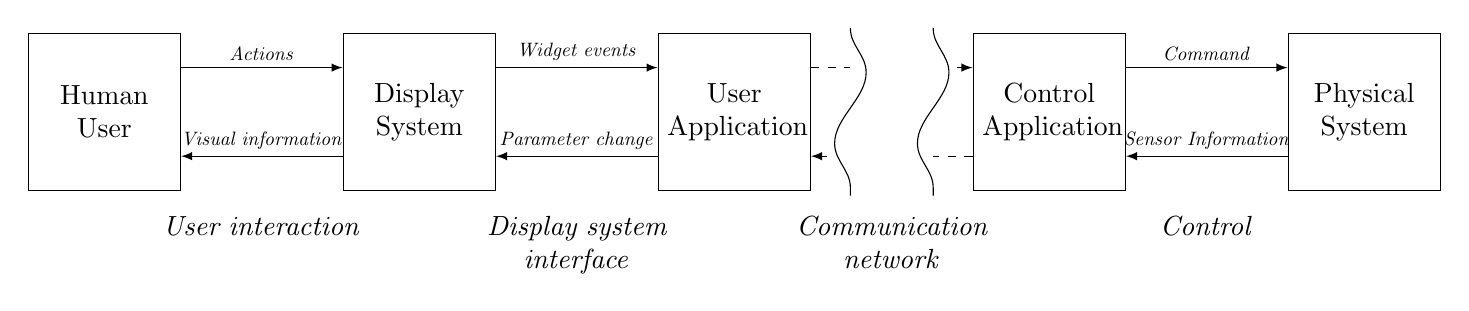
\begin{tikzpicture}

\node[architectureelement] (S1) at (0cm,0cm) {Human \\ User};
\node[architectureelement] (S2) at (4cm,0cm) {Display \\ System};
\node[architectureelement] (S3) at (8cm,0cm) {User \\ Application};
\node[architectureelement] (S4) at (12cm,0cm) {Control \\ Application};
\node[architectureelement] (S5) at (16cm,0cm) {Physical \\ System};

\node[architecturelabel,below] (L1) at (2cm,-1.2cm) {\textit{User interaction}};
\node[architecturelabel,below] (L2) at (6cm,-1.2cm) {\textit{Display system \\ interface}};
\node[architecturelabel,below] (L3) at (10cm,-1.2cm) {\textit{Communication network}};
\node[architecturelabel,below] (L4) at (14cm,-1.2cm) {\textit{Control}};

\coordinate[justright] (S3E1) at (S3.30);
\coordinate[justright] (S3E2) at (S3.-30);
\coordinate[shift={(0.2cm,0cm)}] (S3E2b) at (S3.-30);
\coordinate[justtop] (S3E3) at (S3E1);
\coordinate[justdown] (S3E4) at (S3E2);
\coordinate[justleft] (S4W1) at (S4.150);
\coordinate[shift={(-0.2cm,0cm)}] (S4W1b) at (S4.150);
\coordinate[justleft] (S4W2) at (S4.-150);
\coordinate[justtop] (S4W3) at (S4W1);
\coordinate[justdown] (S4W4) at (S4W2);

\draw[orientedarc] (S1.30) -- (S2.150) node[arclabel, above]{\textit{Actions}};
\draw[orientedarc] (S2.-150) -- (S1.-30) node[arclabel, above]{\textit{Visual information}};

\draw[orientedarc] (S2.30) -- (S3.150) node[arclabel, above]{\textit{Widget events}};
\draw[orientedarc] (S3.-150) -- (S2.-30) node[arclabel, above]{\textit{Parameter change}};

\draw[dashed] (S3.30) -- (S3E1) node[arclabel, above]{\textit{}};
%\draw[loosely dotted] (S3E1) -- (S4W1) node[arclabel, above]{\textit{}};
\draw[orientedarc, dashed] (S4W1b) -- (S4.150) node[arclabel, above]{\textit{}};

\draw[dashed]  (S4.-150) -- (S4W2) node[arclabel, above]{\textit{}};
%\draw[loosely dotted] (S4W2) -- (S3E2) node[arclabel, above]{\textit{}};
\draw[orientedarc, dashed] (S3E2b) -- (S3.-30) node[arclabel, above]{\textit{}};

\draw[breakline] (S3E3) -- (S3E4) node[arclabel, above]{\textit{}};
\draw[breakline] (S4W3) -- (S4W4) node[arclabel, above]{\textit{}};

\draw[orientedarc] (S4.30) -- (S5.150) node[arclabel, above]{\textit{Command}};
\draw[orientedarc] (S5.-150) -- (S4.-30) node[arclabel, above]{\textit{Sensor Information}};


\end{tikzpicture}
}

\caption{Aircraft UIs architecture}
\label{fig:architecture}
\end{figure*}




  % ==<< Section >>===================================================
  \section{State of the art}
  As of today, in order to pass qualification, UIs must undergo a massive, long test procedure, like many other pieces of embedded software. However, the fact that UIs interact directly with humans makes the conception process much heavier. Indeed, fully automatic generation of UIs still does not yield satisfactory results, and extensive automatic testing is not possible (see Fig.~\ref{fig:process1}).

  As a consequence, UIs have to be tested manually during the verification and validation phases. Since these tests happen at the end of the conception loop, errors found during manual tests can become excessively costly to correct, needing to get back in the conception loop.

\begin{figure}[H]
\centering
\resizebox{\linewidth}{!}{
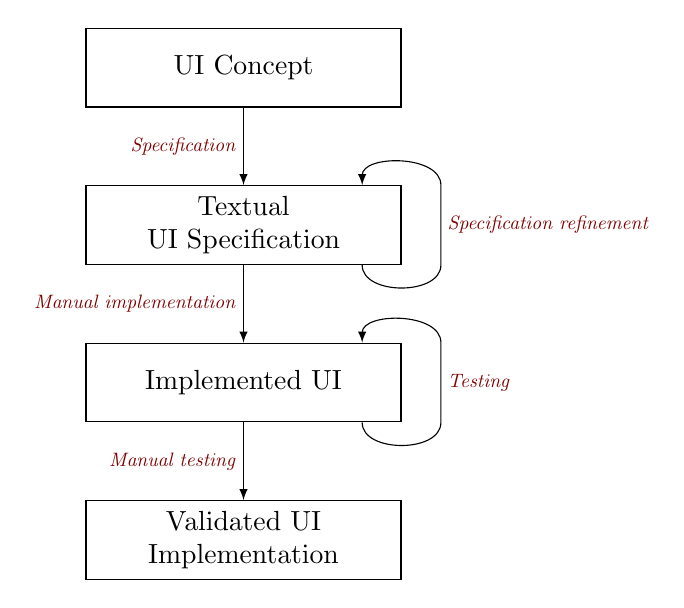
\begin{tikzpicture}

\node[processstep] (S1) at (0cm,6cm) {UI Concept};
\node[processstep] (S2) at (0cm,4cm) {Textual \\ UI Specification};
\node[processstep] (S3) at (0cm,2cm) {Implemented UI};
\node[processstep] (S4) at (0cm,0cm) {Validated UI \\ Implementation};

\coordinate[justright] (S2NORTHEAST1) at (S2.north east);
\coordinate[justright] (S2SOUTHEAST1) at (S2.south east);
\coordinate[justleft] (S2NORTHEAST2) at (S2.north east);
\coordinate[justleft] (S2SOUTHEAST2) at (S2.south east);

\coordinate[justright] (S3NORTHEAST1) at (S3.north east);
\coordinate[justright] (S3SOUTHEAST1) at (S3.south east);
\coordinate[justleft] (S3NORTHEAST2) at (S3.north east);
\coordinate[justleft] (S3SOUTHEAST2) at (S3.south east);

\draw[orientedarc] (S1) -- (S2) node[arclabelred, left]{\textit{Specification}};
\draw[orientedarc] (S2) -- (S3) node[arclabelred, left]{\textit{Manual implementation}};
\draw[orientedarc] (S3) -- (S4) node[arclabelred, left]{\textit{Manual testing}};
\draw[orientedarc] (S2SOUTHEAST2) to[bend right=90] (S2SOUTHEAST1) -- (S2NORTHEAST1) node[arclabelred, right]{\textit{Specification refinement}} to[bend right=90] (S2NORTHEAST2);
\draw[orientedarc] (S3SOUTHEAST2) to[bend right=90] (S3SOUTHEAST1) -- (S3NORTHEAST1) node[arclabelred, right]{\textit{Testing}} to[bend right=90] (S3NORTHEAST2);

\end{tikzpicture}
}

\caption{Classical UI conception process}
\label{fig:process1}
\end{figure}

New tools have been developed in order to enhance this heavy process. Some of these tools can be used in order to generate an abstract model of the UI, taking its code as an input, allowing to perform formal validation on the implemented UI \cite{cortier2008}. Other methods allow to specify UIs using specific languages in order to validate critical parts \cite{madani2007}.

However, a common language allowing an efficient collaboration of these different tools does not exist yet. As a consequence, critical UIs development process can become complex and costly (see Fig~\ref{fig:process2}). 



\begin{figure}[H]
\centering
\resizebox{\linewidth}{!}{
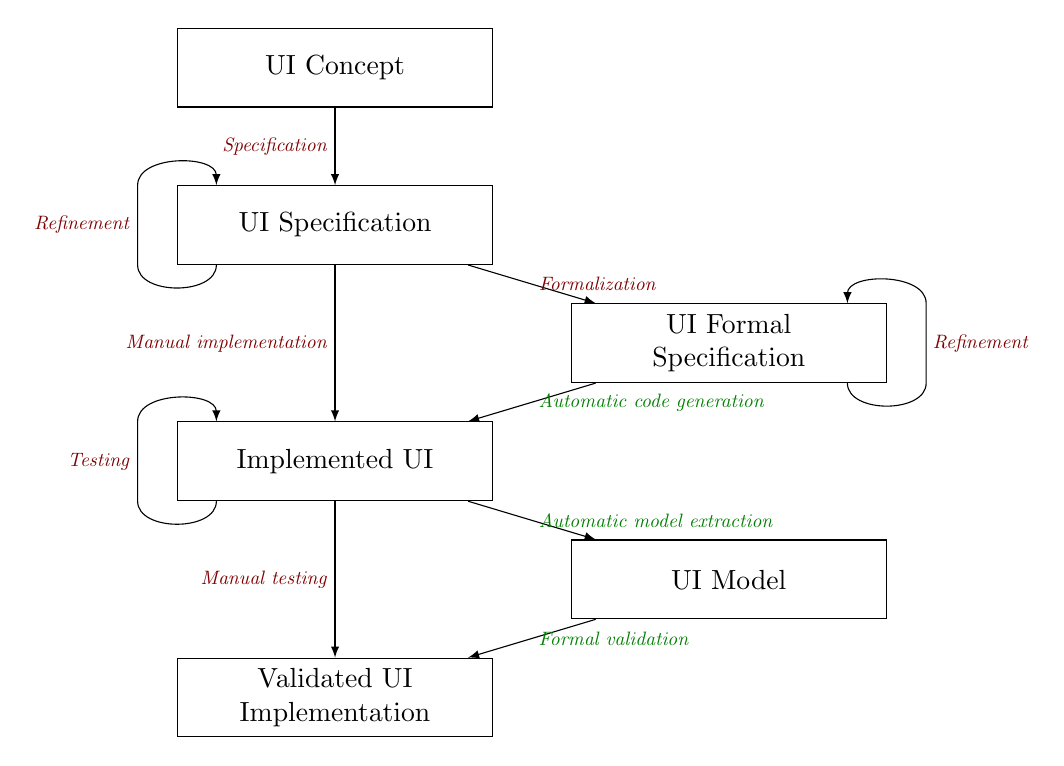
\begin{tikzpicture}
\node[processstep] (S1) at (0cm,8cm) {UI Concept};
\node[processstep] (S2) at (0cm,6cm) {UI Specification};
\node[processstep] (S3) at (0cm,3cm) {Implemented UI};
\node[processstep] (S4) at (0cm,0cm) {Validated UI \\ Implementation};
\node[processstep] (S5) at (5cm,4.5cm) {UI Formal \\ Specification};
\node[processstep] (S6) at (5cm,1.5cm) {UI Model};

\coordinate[justleft] (S2NORTHEAST1) at (S2.north west);
\coordinate[justleft] (S2SOUTHEAST1) at (S2.south west);
\coordinate[justright] (S2NORTHEAST2) at (S2.north west);
\coordinate[justright] (S2SOUTHEAST2) at (S2.south west);

\coordinate[justleft] (S3NORTHEAST1) at (S3.north west);
\coordinate[justleft] (S3SOUTHEAST1) at (S3.south west);
\coordinate[justright] (S3NORTHEAST2) at (S3.north west);
\coordinate[justright] (S3SOUTHEAST2) at (S3.south west);

\coordinate[justright] (S5NORTHEAST1) at (S5.north east);
\coordinate[justright] (S5SOUTHEAST1) at (S5.south east);
\coordinate[justleft] (S5NORTHEAST2) at (S5.north east);
\coordinate[justleft] (S5SOUTHEAST2) at (S5.south east);

\draw[orientedarc] (S1) -- (S2) node[arclabelred, left]{\textit{Specification}};
\draw[orientedarc] (S2) -- (S3) node[arclabelred, left]{\textit{Manual implementation}};
\draw[orientedarc] (S3) -- (S4) node[arclabelred, left]{\textit{Manual testing}};
\draw[orientedarc] (S2SOUTHEAST2) to[bend left=90] (S2SOUTHEAST1) -- (S2NORTHEAST1) node[arclabelred, left]{\textit{Refinement}} to[bend left=90] (S2NORTHEAST2);
\draw[orientedarc] (S3SOUTHEAST2) to[bend left=90] (S3SOUTHEAST1) -- (S3NORTHEAST1) node[arclabelred, left]{\textit{Testing}} to[bend left=90] (S3NORTHEAST2);
\draw[orientedarc] (S2) -- (S5) node[arclabelred, right]{\textit{Formalization}};
\draw[orientedarc] (S5) -- (S3) node[arclabelgreen, right]{\textit{Automatic code generation}};
\draw[orientedarc] (S5SOUTHEAST2) to[bend right=90] (S5SOUTHEAST1) -- (S5NORTHEAST1) node[arclabelred, right]{\textit{Refinement}} to[bend right=90] (S5NORTHEAST2);

\draw[orientedarc] (S3) -- (S6) node[arclabelgreen, right]{\textit{Automatic model extraction}};
\draw[orientedarc] (S6) -- (S4) node[arclabelgreen, right]{\textit{Formal validation}};

\end{tikzpicture}

}

\caption{State-of-the-art UI conception process}
\label{fig:process2}
\end{figure}


 % ==<< Section >>===================================================
 \section{Thesis objectives}
Progress toward a straightforward conception process (see Fig~\ref{fig:process3}) is required to the conception of future UIs. The existence of a formal language taking into account all the aspects of critical UIs (see Fig~\ref{fig:domains}) would greatly help to fulfil this goal.

This formal language would take into account the different aspects of UIs :
\begin{itemize}
\item{Static aspects:}
	\begin{itemize}
	\item{Structure}
	\item{Look \& Feel}
	\end{itemize}
\item{Dynamic aspects:} 
\begin{itemize}
	\item{Behaviour}
	\item{Human interaction}
	\item{System interface}
\end{itemize}
\end{itemize}

This language should also integrate the aspects of critical embedded systems :
\begin{itemize}
\item{Embedded systems}
	\begin{itemize}
	\item{Ressources footprint}
	\item{Timing aspects}
	\end{itemize}
\item{Dependability:} 
\begin{itemize}
	\item{Reliability}
	\item{Integrity}
	\item{Availability}
\end{itemize}
\end{itemize}




\begin{figure}[H]
\centering
\resizebox{\linewidth}{!}{
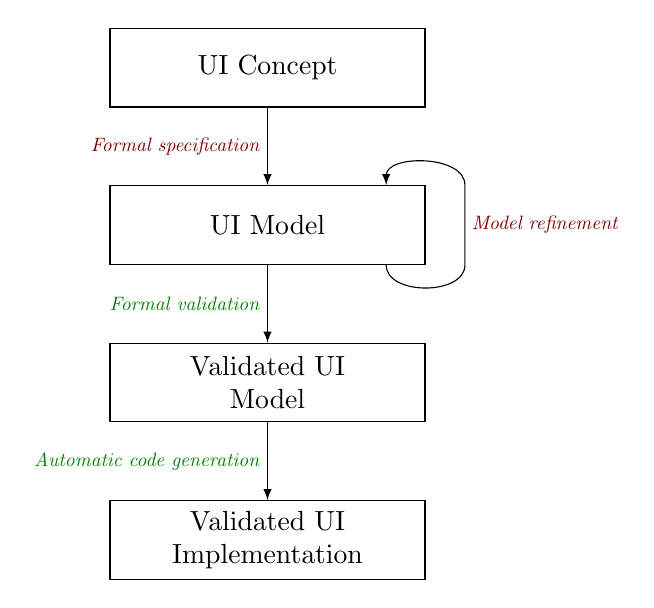
\begin{tikzpicture}

\node[processstep] (S1) at (0cm,6cm) {UI Concept};
\node[processstep] (S2) at (0cm,4cm) {UI Model};
\node[processstep] (S3) at (0cm,2cm) {Validated UI \\ Model};
\node[processstep] (S4) at (0cm,0cm) {Validated UI \\ Implementation};

\coordinate[justright] (S2NORTHEAST1) at (S2.north east);
\coordinate[justright] (S2SOUTHEAST1) at (S2.south east);
\coordinate[justleft] (S2NORTHEAST2) at (S2.north east);
\coordinate[justleft] (S2SOUTHEAST2) at (S2.south east);

\draw[orientedarc] (S1) -- (S2) node[arclabelred, left]{\textit{Formal specification}};
\draw[orientedarc] (S2) -- (S3) node[arclabelgreen, left]{\textit{Formal validation}};
\draw[orientedarc] (S3) -- (S4) node[arclabelgreen, left]{\textit{Automatic code generation}};
\draw[orientedarc] (S2SOUTHEAST2) to[bend right=90] (S2SOUTHEAST1) -- (S2NORTHEAST1) node[arclabelred, right]{\textit{Model refinement}} to[bend right=90] (S2NORTHEAST2);

\end{tikzpicture}
}

\caption{Proposed UI conception process}
\label{fig:process3}
\end{figure}



  % ==<< Section >>===================================================
  \section{Titre 3}
  Sed aliquam varius dui vitae dapibus. Pellentesque eget est sagittis velit blandit fringilla. Sed adipiscing odio at orci tempor tincidunt sed. Praesent lectus lacus, suscipit vitae volutpat ut, sagittis a augue. Ut elit velit, tristique sit amet consectetur id, mollis vel mi. Maecenas congue varius purus, suscipit sagittis tellus adipiscing eget figure~\ref{fig:figure1}.

  
  Nulla risus nisl, dictum non dictum ornare, tincidunt vitae urna. Proin accumsan nisl nibh, venenatis ornare urna. Nullam metus enim, malesuada eget condimentum nec, tincidunt nec arcu. In eget nibh leo. In sem lectus, ultrices ac semper at, gravida ut justo. Nullam condimentum egestas ligula non rutrum. Vivamus at metus libero, congue pretium libero. 

  % ==<< Section >>===================================================
  \section{Titre 4}

  % --<< Sous section >>----------------------------------------------
  \subsection{Sous-titre 1}
  Aenean tempor mauris sodales nulla blandit at ultrices arcu pretium. Sed egestas felis in augue congue hendrerit.
  \begin{equation}
    f(x) = ax + b
    \label{equation1}
  \end{equation}
  % Equation numerotee

  Vestibulum risus augue formulae~\eqref{equation1}, convallis quis luctus sed, fringilla quis sapien. Quisque ut ultrices odio. Proin convallis pulvinar elementum. Suspendisse potenti.
  \begin{equation*}
    f(y) = cy + d
  \end{equation*}
  % Equation non numerotee

  % --<< Sous section >>----------------------------------------------
  \subsection{Sous-titre 2}
  Etiam placerat imperdiet lectus, eget placerat est commodo eu. In rhoncus tellus non urna lobortis elementum. Curabitur vestibulum dictum dui et pharetra. Fusce diam tortor, vestibulum vitae sodales nec, fringilla eu enim.


  \begin{table}[H]
    \centering
    \begin{tabular}{|lr|c|c|}
      \hline
      \multicolumn{2}{|l|}{\textbf{Intitule 1}} & \textbf{Intitule 2} & \textbf{Intitule 3} \\
      \hline
      \hline
      item1 & A & 10 & 5 \\
      item2 & B & 20 & 4 \\
      item3 & C & 30 & 3 \\
      \hline
    \end{tabular}
    \caption{Legende du tableau}
    \label{tab:tableau}
  \end{table}
  % Tableau

  % ==<< Section >>===================================================
  \section{Titre 5}
  Phasellus vitae tortor erat. Proin metus neque, condimentum varius volutpat ac, posuere ultrices sapien.

  Donec at elementum enim. Proin feugiat libero ac justo lacinia in lacinia metus malesuada. In ipsum lacus, consectetur sit amet ornare a, placerat at tortor. Aliquam eu est malesuada massa hendrerit cursus. Vestibulum a gravida tellus. Aenean nec tellus sed metus dignissim semper\footnote{Nulla quis elit vel magna sodales malesuada. Phasellus semper libero sit amet eros semper et blandit arcu rhoncus.}.

\end{content}

% Bibliographie au format bibtex dans le fichier jdt-tis.bib
\bibliography{These}

\end{document}
